\documentclass[12pt]{article}
%Fall 2022
% Some basic packages
\usepackage{standalone}[subpreambles=true]
\usepackage[utf8]{inputenc}
\usepackage[T1]{fontenc}
\usepackage{textcomp}
\usepackage[english]{babel}
\usepackage{url}
\usepackage{graphicx}
%\usepackage{quiver}
\usepackage{float}
\usepackage{enumitem}
\usepackage{lmodern}
\usepackage{comment}
\usepackage{hyperref}
\usepackage[usenames,svgnames,dvipsnames]{xcolor}
\usepackage[margin=1in]{geometry}
\usepackage{pdfpages}

\pdfminorversion=7

% Don't indent paragraphs, leave some space between them
\usepackage{parskip}

% Hide page number when page is empty
\usepackage{emptypage}
\usepackage{subcaption}
\usepackage{multicol}
\usepackage[b]{esvect}

% Math stuff
\usepackage{amsmath, amsfonts, mathtools, amsthm, amssymb}
\usepackage{bbm}
\usepackage{stmaryrd}
\allowdisplaybreaks

% Fancy script capitals
\usepackage{mathrsfs}
\usepackage{cancel}
% Bold math
\usepackage{bm}
% Some shortcuts
\newcommand{\rr}{\ensuremath{\mathbb{R}}}
\newcommand{\zz}{\ensuremath{\mathbb{Z}}}
\newcommand{\qq}{\ensuremath{\mathbb{Q}}}
\newcommand{\nn}{\ensuremath{\mathbb{N}}}
\newcommand{\ff}{\ensuremath{\mathbb{F}}}
\newcommand{\cc}{\ensuremath{\mathbb{C}}}
\newcommand{\ee}{\ensuremath{\mathbb{E}}}
\newcommand{\hh}{\ensuremath{\mathbb{H}}}
\renewcommand\O{\ensuremath{\emptyset}}
\newcommand{\norm}[1]{{\left\lVert{#1}\right\rVert}}
\newcommand{\dbracket}[1]{{\left\llbracket{#1}\right\rrbracket}}
\newcommand{\ve}[1]{{\bm{#1}}}
\newcommand\allbold[1]{{\boldmath\textbf{#1}}}
\DeclareMathOperator{\lcm}{lcm}
\DeclareMathOperator{\im}{im}
\DeclareMathOperator{\coim}{coim}
\DeclareMathOperator{\dom}{dom}
\DeclareMathOperator{\tr}{tr}
\DeclareMathOperator{\rank}{rank}
\DeclareMathOperator*{\var}{Var}
\DeclareMathOperator*{\ev}{E}
\DeclareMathOperator{\dg}{deg}
\DeclareMathOperator{\aff}{aff}
\DeclareMathOperator{\conv}{conv}
\DeclareMathOperator{\inte}{int}
\DeclareMathOperator*{\argmin}{argmin}
\DeclareMathOperator*{\argmax}{argmax}
\DeclareMathOperator{\graph}{graph}
\DeclareMathOperator{\sgn}{sgn}
\DeclareMathOperator*{\Rep}{Rep}
\DeclareMathOperator{\Proj}{Proj}
\DeclareMathOperator{\mat}{mat}
\DeclareMathOperator{\diag}{diag}
\DeclareMathOperator{\aut}{Aut}
\DeclareMathOperator{\gal}{Gal}
\DeclareMathOperator{\inn}{Inn}
\DeclareMathOperator{\edm}{End}
\DeclareMathOperator{\Hom}{Hom}
\DeclareMathOperator{\ext}{Ext}
\DeclareMathOperator{\tor}{Tor}
\DeclareMathOperator{\Span}{Span}
\DeclareMathOperator{\Stab}{Stab}
\DeclareMathOperator{\cont}{cont}
\DeclareMathOperator{\Ann}{Ann}
\DeclareMathOperator{\Div}{div}
\DeclareMathOperator{\curl}{curl}
\DeclareMathOperator{\nat}{Nat}
\DeclareMathOperator{\gr}{Gr}
\DeclareMathOperator{\vect}{Vect}
\DeclareMathOperator{\id}{id}
\DeclareMathOperator{\Mod}{Mod}
\DeclareMathOperator{\sign}{sign}
\DeclareMathOperator{\Surf}{Surf}
\DeclareMathOperator{\fcone}{fcone}
\DeclareMathOperator{\Rot}{Rot}
\DeclareMathOperator{\grad}{grad}
\DeclareMathOperator{\atan2}{atan2}
\DeclareMathOperator{\Ric}{Ric}
\let\vec\relax
\DeclareMathOperator{\vec}{vec}
\let\Re\relax
\DeclareMathOperator{\Re}{Re}
\let\Im\relax
\DeclareMathOperator{\Im}{Im}
% Put x \to \infty below \lim
\let\svlim\lim\def\lim{\svlim\limits}

%wide hat
\usepackage{scalerel,stackengine}
\stackMath
\newcommand*\wh[1]{%
\savestack{\tmpbox}{\stretchto{%
  \scaleto{%
    \scalerel*[\widthof{\ensuremath{#1}}]{\kern-.6pt\bigwedge\kern-.6pt}%
    {\rule[-\textheight/2]{1ex}{\textheight}}%WIDTH-LIMITED BIG WEDGE
  }{\textheight}% 
}{0.5ex}}%
\stackon[1pt]{#1}{\tmpbox}%
}
\parskip 1ex

%Make implies and impliedby shorter
\let\implies\Rightarrow
\let\impliedby\Leftarrow
\let\iff\Leftrightarrow
\let\epsilon\varepsilon

% Add \contra symbol to denote contradiction
\usepackage{stmaryrd} % for \lightning
\newcommand\contra{\scalebox{1.5}{$\lightning$}}

% \let\phi\varphi

% Command for short corrections
% Usage: 1+1=\correct{3}{2}

\definecolor{correct}{HTML}{009900}
\newcommand\correct[2]{\ensuremath{\:}{\color{red}{#1}}\ensuremath{\to }{\color{correct}{#2}}\ensuremath{\:}}
\newcommand\green[1]{{\color{correct}{#1}}}

% horizontal rule
\newcommand\hr{
    \noindent\rule[0.5ex]{\linewidth}{0.5pt}
}

% hide parts
\newcommand\hide[1]{}

% si unitx
\usepackage{siunitx}
\sisetup{locale = FR}

%allows pmatrix to stretch
\makeatletter
\renewcommand*\env@matrix[1][\arraystretch]{%
  \edef\arraystretch{#1}%
  \hskip -\arraycolsep
  \let\@ifnextchar\new@ifnextchar
  \array{*\c@MaxMatrixCols c}}
\makeatother

\renewcommand{\arraystretch}{0.8}

\renewcommand{\baselinestretch}{1.5}

\usepackage{graphics}
\usepackage{epstopdf}

\RequirePackage{hyperref}
%%
%% Add support for color in order to color the hyperlinks.
%% 
\hypersetup{
  colorlinks = true,
  urlcolor = blue,
  citecolor = blue
}
%%fakesection Links
\hypersetup{
    colorlinks,
    linkcolor={red!50!black},
    citecolor={green!50!black},
    urlcolor={blue!80!black}
}
%customization of cleveref
\RequirePackage[capitalize,nameinlink]{cleveref}[0.19]

% Per SIAM Style Manual, "section" should be lowercase
\crefname{section}{section}{sections}
\crefname{subsection}{subsection}{subsections}
\Crefname{section}{Section}{Sections}
\Crefname{subsection}{Subsection}{Subsections}

% Per SIAM Style Manual, "Figure" should be spelled out in references
\Crefname{figure}{Figure}{Figures}

% Per SIAM Style Manual, don't say equation in front on an equation.
\crefformat{equation}{\textup{#2(#1)#3}}
\crefrangeformat{equation}{\textup{#3(#1)#4--#5(#2)#6}}
\crefmultiformat{equation}{\textup{#2(#1)#3}}{ and \textup{#2(#1)#3}}
{, \textup{#2(#1)#3}}{, and \textup{#2(#1)#3}}
\crefrangemultiformat{equation}{\textup{#3(#1)#4--#5(#2)#6}}%
{ and \textup{#3(#1)#4--#5(#2)#6}}{, \textup{#3(#1)#4--#5(#2)#6}}{, and \textup{#3(#1)#4--#5(#2)#6}}

% But spell it out at the beginning of a sentence.
\Crefformat{equation}{#2Equation~\textup{(#1)}#3}
\Crefrangeformat{equation}{Equations~\textup{#3(#1)#4--#5(#2)#6}}
\Crefmultiformat{equation}{Equations~\textup{#2(#1)#3}}{ and \textup{#2(#1)#3}}
{, \textup{#2(#1)#3}}{, and \textup{#2(#1)#3}}
\Crefrangemultiformat{equation}{Equations~\textup{#3(#1)#4--#5(#2)#6}}%
{ and \textup{#3(#1)#4--#5(#2)#6}}{, \textup{#3(#1)#4--#5(#2)#6}}{, and \textup{#3(#1)#4--#5(#2)#6}}

% Make number non-italic in any environment.
\crefdefaultlabelformat{#2\textup{#1}#3}

% Environments
\makeatother
% For box around Definition, Theorem, \ldots
%%fakesection Theorems
\usepackage{thmtools}
\usepackage[framemethod=TikZ]{mdframed}

\theoremstyle{definition}
\mdfdefinestyle{mdbluebox}{%
	roundcorner = 10pt,
	linewidth=1pt,
	skipabove=12pt,
	innerbottommargin=9pt,
	skipbelow=2pt,
	nobreak=true,
	linecolor=blue,
	backgroundcolor=TealBlue!5,
}
\declaretheoremstyle[
	headfont=\sffamily\bfseries\color{MidnightBlue},
	mdframed={style=mdbluebox},
	headpunct={\\[3pt]},
	postheadspace={0pt}
]{thmbluebox}

\mdfdefinestyle{mdredbox}{%
	linewidth=0.5pt,
	skipabove=12pt,
	frametitleaboveskip=5pt,
	frametitlebelowskip=0pt,
	skipbelow=2pt,
	frametitlefont=\bfseries,
	innertopmargin=4pt,
	innerbottommargin=8pt,
	nobreak=false,
	linecolor=RawSienna,
	backgroundcolor=Salmon!5,
}
\declaretheoremstyle[
	headfont=\bfseries\color{RawSienna},
	mdframed={style=mdredbox},
	headpunct={\\[3pt]},
	postheadspace={0pt},
]{thmredbox}

\declaretheorem[%
style=thmbluebox,name=Theorem,numberwithin=section]{thm}
\declaretheorem[style=thmbluebox,name=Lemma,sibling=thm]{lem}
\declaretheorem[style=thmbluebox,name=Proposition,sibling=thm]{prop}
\declaretheorem[style=thmbluebox,name=Corollary,sibling=thm]{coro}
\declaretheorem[style=thmredbox,name=Example,sibling=thm]{eg}

\mdfdefinestyle{mdgreenbox}{%
	roundcorner = 10pt,
	linewidth=1pt,
	skipabove=12pt,
	innerbottommargin=9pt,
	skipbelow=2pt,
	nobreak=true,
	linecolor=ForestGreen,
	backgroundcolor=ForestGreen!5,
}

\declaretheoremstyle[
	headfont=\bfseries\sffamily\color{ForestGreen!70!black},
	bodyfont=\normalfont,
	spaceabove=2pt,
	spacebelow=1pt,
	mdframed={style=mdgreenbox},
	headpunct={ --- },
]{thmgreenbox}

\declaretheorem[style=thmgreenbox,name=Definition,sibling=thm]{defn}

\mdfdefinestyle{mdgreenboxsq}{%
	linewidth=1pt,
	skipabove=12pt,
	innerbottommargin=9pt,
	skipbelow=2pt,
	nobreak=true,
	linecolor=ForestGreen,
	backgroundcolor=ForestGreen!5,
}
\declaretheoremstyle[
	headfont=\bfseries\sffamily\color{ForestGreen!70!black},
	bodyfont=\normalfont,
	spaceabove=2pt,
	spacebelow=1pt,
	mdframed={style=mdgreenboxsq},
	headpunct={},
]{thmgreenboxsq}
\declaretheoremstyle[
	headfont=\bfseries\sffamily\color{ForestGreen!70!black},
	bodyfont=\normalfont,
	spaceabove=2pt,
	spacebelow=1pt,
	mdframed={style=mdgreenboxsq},
	headpunct={},
]{thmgreenboxsq*}

\mdfdefinestyle{mdblackbox}{%
	skipabove=8pt,
	linewidth=3pt,
	rightline=false,
	leftline=true,
	topline=false,
	bottomline=false,
	linecolor=black,
	backgroundcolor=RedViolet!5!gray!5,
}
\declaretheoremstyle[
	headfont=\bfseries,
	bodyfont=\normalfont\small,
	spaceabove=0pt,
	spacebelow=0pt,
	mdframed={style=mdblackbox}
]{thmblackbox}

\theoremstyle{plain}
\declaretheorem[name=Question,sibling=thm,style=thmblackbox]{ques}
\declaretheorem[name=Remark,sibling=thm,style=thmgreenboxsq]{remark}
\declaretheorem[name=Remark,sibling=thm,style=thmgreenboxsq*]{remark*}
\newtheorem{ass}[thm]{Assumptions}

\theoremstyle{definition}
\newtheorem*{problem}{Problem}
\newtheorem{claim}[thm]{Claim}
\theoremstyle{remark}
\newtheorem*{case}{Case}
\newtheorem*{notation}{Notation}
\newtheorem*{note}{Note}
\newtheorem*{motivation}{Motivation}
\newtheorem*{intuition}{Intuition}
\newtheorem*{conjecture}{Conjecture}

% Make section starts with 1 for report type
%\renewcommand\thesection{\arabic{section}}

% End example and intermezzo environments with a small diamond (just like proof
% environments end with a small square)
\usepackage{etoolbox}
\AtEndEnvironment{vb}{\null\hfill$\diamond$}%
\AtEndEnvironment{intermezzo}{\null\hfill$\diamond$}%
% \AtEndEnvironment{opmerking}{\null\hfill$\diamond$}%

% Fix some spacing
% http://tex.stackexchange.com/questions/22119/how-can-i-change-the-spacing-before-theorems-with-amsthm
\makeatletter
\def\thm@space@setup{%
  \thm@preskip=\parskip \thm@postskip=0pt
}

% Fix some stuff
% %http://tex.stackexchange.com/questions/76273/multiple-pdfs-with-page-group-included-in-a-single-page-warning
\pdfsuppresswarningpagegroup=1


% My name
\author{Jaden Wang}



\begin{document}
\centerline {\textsf{\textbf{\LARGE{Homework 3}}}}
\centerline {Jaden Wang}
\vspace{.15in}

\begin{problem}[1]
Recall that since $ \lambda_i \geq 0$ and $ h_i(x) \leq 0$ for all $ x$ and  $ i$, we have $ \sum \lambda_i h_i(x) \leq 0$. Consider the first inequality when we choose $ \lambda_i =0$ for all $ i$, we have
\begin{align*}
	0=\sum \lambda_i h_i(x^* ) \leq \sum \lambda_i^* h_i(x^* ) \leq 0
\end{align*}
This forces $ \sum \lambda_i^* h_i(x^* ) = 0$. Since each $ \lambda_i^* h_i(x^* ) \leq 0$, it must be that $ \lambda_i^* h_i(x^* ) = 0$.

Now consider the second inequality where we choose $ \lambda_i \geq 0$ s.t.\ $ \lambda_i h_i(x^* ) = \lambda_i^* h_i(x)$. This is possible because $ h_i \leq 0$.
\begin{align*}
	\mathscr{L}(x^* ,\lambda^* ) &\leq \mathscr{L}(x,\lambda^* )  \\
	f(x^* ) + \sum \lambda_i^* h_i(x^* ) &\leq f(x) + \sum \lambda_ih_i(x)\\
	f(x^* ) &\leq f(x) + \sum \lambda_i^* (h_i(x)-h_i(x^* ))\\
		&\leq f(x) + \underbrace{ \sum \lambda_i^* h_i(x) - \sum \lambda_i h_i(x^* )}_{=0 } && \text{1st inequality} \\
		&\leq f(x)
\end{align*}
\end{problem}

\begin{problem}[2]
Substituting $ \lambda^* =(1,0)$, the Lagrangian becomes
\begin{align*}
	\mathscr{L}(x_1,x_2) = x_1^2-x_1+x_2^2+x_2+1.
\end{align*}
Then
\begin{align*}
	\nabla \mathscr{L} = \begin{pmatrix} 2x_1-1\\2x_2+1 \end{pmatrix} \text{ and } \nabla ^2 \mathscr{L} = \begin{pmatrix} 2&0\\0&2 \end{pmatrix} \succ 0
\end{align*}
Since the Hessian is already positive definite, it satisfies the 2nd order condition on the null space of $ h_1'\left( \frac{1}{2},-\frac{1}{2} \right) $.
\end{problem}

\begin{problem}[3]
To maximize distance, we need to maximize the integral of velocity with respect to time. We are asked to express $ dt$ in terms of  $ dm$ and thrust  $ T$ in terms of other variables. We see that
\begin{align*}
	dt = \frac{m\ dv}{ T-D} &= - \frac{c\ dm}{ T} \\
	\frac{1}{T} &= \frac{1}{D} \left( 1+ \frac{m\ dv}{ c\ dm} \right) 
\end{align*}
Therefore,
\begin{align*}
	x(t_f) - x(0) &= \int_{ 0}^{ t_f} v(t) dt   \\
	&= \int_{ m_0}^{ m_f} - \frac{ cv}{ T} dm   \\
	&= \int_{ m_f}^{ m_0} \frac{c v}{ T} dm \\
	&= \int_{ m_f}^{ m_0}\frac{c v}{ D} \left( 1+ \frac{m\ dv}{ c\ dm} \right)    
\end{align*}
\end{problem}

\begin{problem}[4]
\begin{enumerate}[label=(\roman*)]
	\item By conservation of energy, we have
		\begin{align*}
			K = \frac{1}{2} m v_f^2 &= mgb = T \\
			v_f &= \sqrt{2gb}  
		\end{align*}
	Since we have constant acceleration induced by gravity, the average velocity must be half of $ v_f$. Thus
	 \begin{align*}
		t_f-0 = \frac{d}{\frac{1}{2}v_f} = \sqrt{\frac{2(a^2+b^2)}{gb }}.
	\end{align*}
\item More generally, the conservation of energy gives
	\begin{align*}
		\frac{1}{2} m v(x) &= mgy(x) \\
		v(x) &= \sqrt{2g y(x)}  
	\end{align*}
	We also know that arc length has differential $ ds = \sqrt{1+\dot{y}(x)^2} dx = v(x(t)) dt$. Thus we have
	\begin{align*}
		t &= \int_{ t_0}^{ t_f} dt   \\
		t(y)  &= \int_{ 0}^{ a} \sqrt{\frac{1+\dot{y}(x)^2}{2gy(x)}} dx  
	\end{align*}
	The Euler-Lagrange gives $ y(1+\dot{y}^2) = $const. Plugging in the solutions we have $ \dot{y}(x) = \frac{d y}{d x} = \frac{d y}{d \psi} \frac{d \psi}{d x} = - \frac{\sin \psi}{ 1+\cos \psi} $ and
	\begin{align*}
		\beta(1+\cos \psi)\left( 1+ \frac{\sin^2 \psi}{ (1+ \cos \psi)^2} \right)  &= \beta \left( 1+ \frac{\cos \psi + \cos^2 \psi + \sin^2\psi}{ 1+ \cos \psi} \right)   \\
		&= 2 \beta = \text{ const} 
	\end{align*}
	Thus this is indeed a solution. Since $ dx = \beta(1+\cos \psi) d \psi$, we have
	\begin{align*}
		t &= \int_{ \psi_1}^{ \psi_2} \sqrt{\frac{1+ \sin^2 \psi / (1+\cos \psi)^2}{ 2g \beta (1+ \cos \psi)}} \beta(1+\cos \psi) d \psi   \\
		&= \int_{ \psi_1}^{ \psi_2} \frac{\beta}{ \sqrt{g \beta} }  d \psi \\
		&= \sqrt{ \frac{\beta}{ g}} (\psi_2 - \psi_1)  
	\end{align*}
\item The boundary conditions tell us  $ \beta(1+\cos \psi_1) = 0$ so $ \cos \psi_1 = -1 \implies \psi_1 = \pi$. Thus
	\begin{align*}
		\alpha + \beta(\sin \psi_1 + \psi_1) &= 0 \\
		\alpha+ \beta(0+ \pi) &= 0 \\
		\pi &= - \frac{ \alpha}{ \beta}
	\end{align*}
	Then we see that letting $ \theta = \psi_2- \psi_1= \psi_2 - \pi$, the boundary condition becomes
	\begin{align*}
		\alpha + \beta(\sin (\theta+\pi)+ \theta + \pi) &= a \\
		\alpha + \beta(-\sin \theta + \theta + \pi) &= a \\
		\theta - \sin \theta &= \frac{a- \alpha}{ \beta} - \pi  \\
		&= \frac{a}{ \beta} \\
		\beta (1+ \cos (\theta+\pi)) &= b \\
		\beta(1-\cos \theta) &= b\\ 
		(1-\cos \theta) &= \frac{b}{\beta} \\
	\end{align*}
	Thus it is clear now that $ \theta$ satisfies
	\begin{align*}
		(1-\cos \theta) - \frac{b}{a} (\theta - \sin \theta) =0
	\end{align*}
	Thus $ \beta = \frac{b}{1-\cos \theta}$ and $ \alpha = - \frac{b\pi}{ 1- \cos \theta}$.
\item If $ a = 4$ and  $ b=2$, then the time for the ramp is $ t_1 = 0.79$s and the time for the cycloid is $ \theta = 3.50837$ and $ t_2 = 0.63$s. That is $ 0.16$s of difference. The distance $ d(t)$ of the ramp is $ d(t) = \frac{1}{2} g \frac{b}{ \sqrt{a^2+b^2} } t^2$. So $ d(t_2) = 2.85$ft. It is clear from this formula that if $ a \gg b$,  $ d(t)$ will be much smaller given a fixed time. 
\end{enumerate}
\end{problem}

\begin{problem}[5]
We see that $ F = \dot{y}(t)^2+12ty(t)$. Euler-Lagrange is
\begin{align*}
	12t &= \frac{d}{dt} (2\dot{y})= 2\ddot{y} \\
	\ddot{y} &= 6t \\
	\dot{y} &= 3t^2+C \\
	y(t) &= t^3+Ct+D 
\end{align*}
Since $ y(0) = 0 = D$ and  $ y(1) = 1+C = 0 \implies C=-1$, we have the candidate minimizer
\begin{align*}
	y^*(t) = t^3-t.
\end{align*}
We see that $ F_r = 2r$,  $ F_{r r} = 2 >0$ so $ y^* $ is regular. Also $ F_{yy}=0, F_{yr}=0$. Let $ f$ be the perturbation with $ f(0)=f(1)=0$ and $ 2 \omega(t, f, \dot{f}) = F_{yy} f^2 + 2F_{yr} f \dot{f} + F_{rr} \dot{f}^2$. Then the Jacobi condition requires
\begin{align*}
	\omega_f &= \omega_{\dot{f} t} + \omega_{\dot{f} f} \dot{f} + \omega_{\dot{f}\dot{f}} \ddot{f} \\
	0 &= \dot{f} \ddot{f} + 0+ \ddot{f} \\
	0&= (1+\dot{f}) \ddot{f} \\
	\dot{f} &= -1 \text{ or } \ddot{f} =0\\
	f(t) &= -t + C \text{ or } f(t) = C_1t +D. 
\end{align*}
But the initial value condition forces $ C=C_1=D=0$ and $ f(t) =-t$ doesn't satisfies  $ f(1)=0$ so it must be that  $ f(t) =0$. We see that between 0 and 1, there is no conjugate point to 0 (we don't have corners when we construct the new $ \phi$ in the proof). Thus Jacobi condition is satisfied for $ y^* $.

Finally, we check Weierstrass condition:
\begin{align*}
	E(t,y,r,q)&= F(t,y,q)-F(t,y,r) -(q-r)F_r(t,y,r) \\ 
	&= q^2+12ty-r^2-12ty - (q-r)2r \\
	&= q^2-r^2-(q-r)2r \\
	&= (q-r)^2 \geq 0 \ \forall \ q,r
\end{align*}
Thus $ y^* $ (and any other function) satisfies the Weierstrass condition. Since $ y^* $ passes all four sufficient conditions, $ y^* $ is a strong local minimizer. Since this is the only candidate for a global minimizer, either it is the global minimizer or the solution doesn't exist. Assuming it is the former, we have
\begin{align*}
	\min J(y) = J(y^* ) &= \int_{ 0}^{ 1} (3t^2-1)^2 +12t(t^3-t) dt \\
	&=\int_{ 0}^{ 1} ( 9t^{4}-6t^2+1 +12 t^{4} - 12 t^2)dt  \\
	&=\int_{ 0}^{ 1} (  21t^{4} -18t^2 + 1) dt \\
	&= \left( \frac{21}{5}t^{5}-6t^{3}+t \right) \bigg|_0^1 \\
	&= -\frac{4}{5} 
\end{align*}
\end{problem}
\begin{problem}[6]
We first apply Euler-Lagrange:
\begin{align*}
	\frac{\partial F}{\partial x} &= \frac{d}{dt} \frac{\partial F}{\partial \dot{x}}\\ 
	6t^2 x + 2t^3 \dot{x} &= \frac{d}{dt} (2t^3x) = 6t^2 x + 2 t^3 \dot{x} 
\end{align*}
which is trivially satisfied by all $ x(t)$. Thus all  $ x(t)$ are extremals. We have
 \begin{align*}
	 \min J &= \int_{ t_0}^{ t_1} (3t^2x^2+2t^3x \dot{x}) dt  \\
	 &= \int_{ t_0}^{ t_1} \frac{d}{dt} \left( t^3 x^2 \right) dt  \\
	 &= t^3 x^2 \bigg|_{t_0}^{t_1} \\
	 &= t_1 ^3 x_1^2 - t_0^3x_0^2 
\end{align*}
\end{problem}
\begin{problem}[7]
\begin{enumerate}[label=(\roman*)]
	\item We have $ \frac{\partial F}{\partial y} =0$ and $ \frac{\partial F}{\partial \dot{y}} = (2\dot{y}^2-1) \cdot 2\dot{y} = 4\dot{y}^3-4\dot{y}$. Thus Euler-Lagrange is
	\begin{align*}
		\frac{d}{dt} \frac{\partial F}{\partial \dot{y}} = (3\dot{y}^2 -1)4 \ddot{y} &= 0 \\
		y(t)&= \begin{cases}
			Ct+D & \ddot{y}=0\\
			\pm \frac{1}{\sqrt{3} }t+C_1 & \dot{y}^2 = \frac{1}{3}\\
		\end{cases}\\
		y(t)&= Ct+D \\
	\end{align*}
Thus the extremals are line segments.
\item We have $ F_r = 4r(r^2-1)$. Let $ p=\dot{y}^* (t^{-})$ and $ q = \dot{y}^* (t^{+})$, and $ p \neq q$. Then by strong Erdmann corner condtions, $ p,q$ must satisfy
	 \begin{align*}
		 p(p^2-1) =q(q^2-1)
	\end{align*}
	and
	\begin{align*}
		F(p)-p F_r(p) &= F(q)-qF_r(q) \\
		(p^2-1)^2 - 4p^2(p^2-1) &= (q^2-1)^2 - 4q^2(q^2-1) \\
		(p^2-1)(p^2-1-4p^2) &= (q^2-1)(q^2-1-4q^2) \\
		(p^2-1)(3p^2+1) &= (q^2-1)(3q^2+1) 
	\end{align*}
	If $ p=0$ then  $ q = \pm 1 \neq p$. But then  $ (p^2-1)(3p^2+1) \neq 0$, a contradiction so $ p \neq 0$. If we assume that $ q^2-1 \neq 0$, then we have
	\begin{align*}
		\frac{p^2-1}{ q^2-1} = \frac{q}{p} &= \frac{3q^2+1}{ 3p^2+1}  \\
		3p^2q + q &= 3pq^2+p \\
		(p-q)(3pq-1) &= 0 \\
		pq &= \frac{1}{3} && p \neq q
	\end{align*}
	But this is symmetric, so substituting this back to the first condition would give $ p=q$, a contradiction. Therefore, it must be that  $ q^2-1 = 0 \implies q = \pm 1$. But the two conditions forces $ p = \pm 1$ as well so the slope must be $ p = -q = \pm 1$. 
\item We know any local minimum must be PWS where each piece has the form $ y(t) = \pm t +d$. Then the figure shows a function $ y^* $ with such form. Then $ F(y^* ,\dot{y}^* ,t) = 0$ and thus $ J(y^* ) = 0$. But since $ F \geq 0$,  $ J(y) \geq 0$ always. So this  $ y^* $ indeed achieves the global minimum.
~\begin{figure}[H]
	\centering
	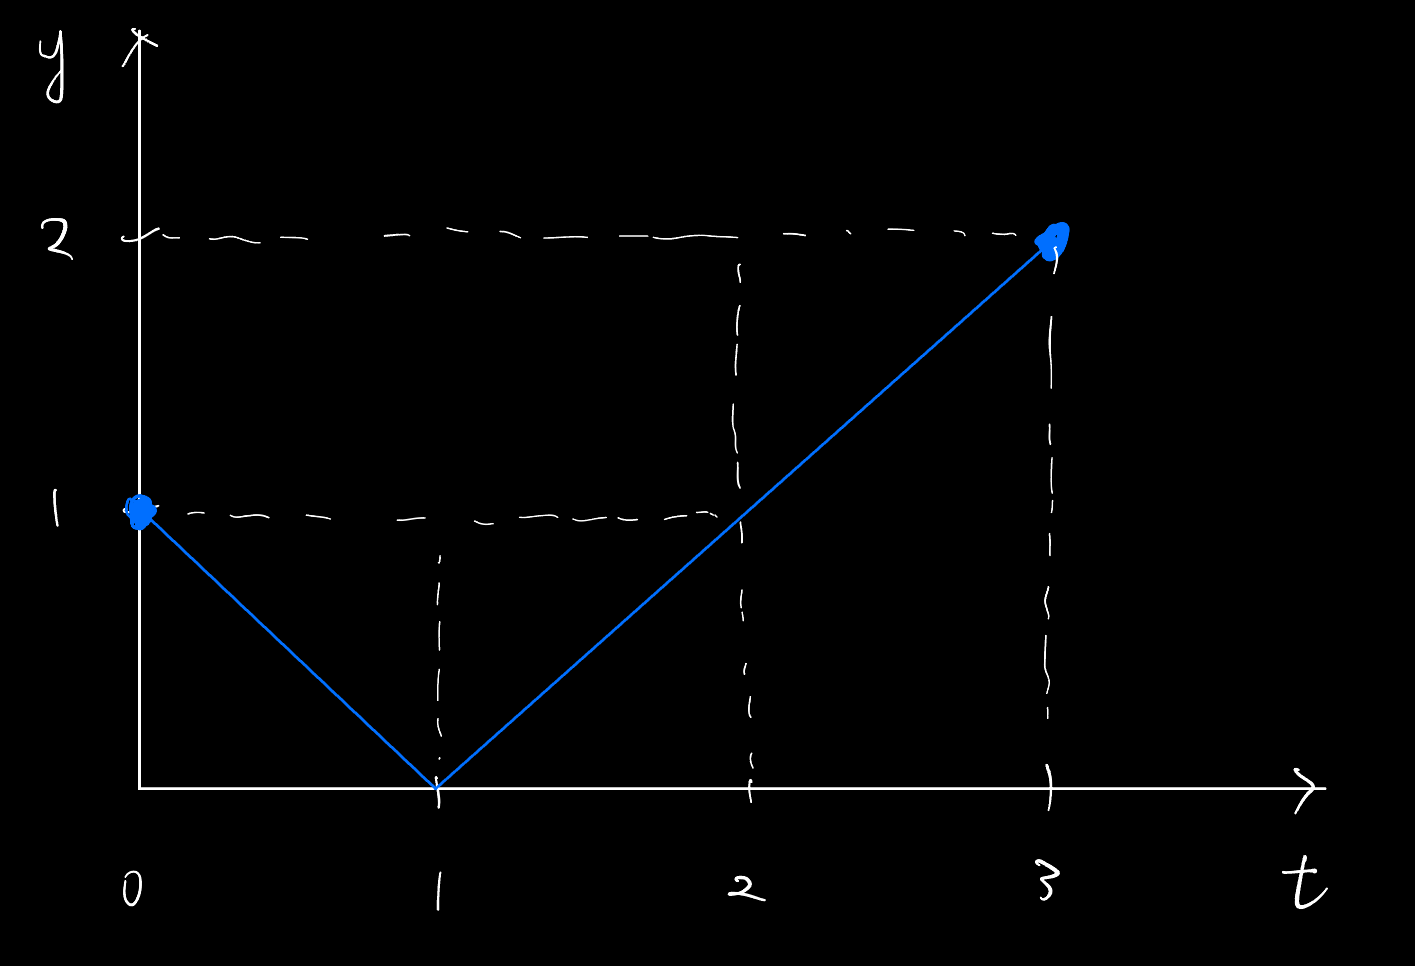
\includegraphics[width=0.6\textwidth]{./figures/pws_sol}
	\caption{A PWS solution with a corner.}
\end{figure}
\item In this case, there is no solution with corners as the figure clearly shows we cannot maintain a slope of $ \pm 1$ to reach  $ y(1)=2$. In the smooth case, the only extremal that satisfies the boundary conditions is  $ y^*=2t$. Then $ \dot{y} = 2$ and $ F_{r r} = 12r-4= 20>0$ so strong Legendre is satisfied.
	For the Jacobi conditions, we have $ F_{yy}=F_{yr}=0$ and let $ f$ be the perturbation with  $ f(t_0)=f(t_1)=0$ and $ 2 \omega = 20 \dot{f}^2$. Then
	\begin{align*}
		0 &= 20 \ddot{f} + 0 + 20 \ddot{f} \\
		\ddot{f} &= 0 \\
		f &\equiv 0 
	\end{align*}
	by the initial conditions. Thus there is no conjugate points as Problem 5.

	Finally, Weierstrass conditions says
	\begin{align*}
		E(t,y,q,r) &=  (q^2-1)^2-(2^2-1)^2-(q-2)4 \cdot 2(2^2-1) \\
		&= q^{4} - 2q^2-24q + 39
	\end{align*}
We see that when $ q = 2$,  $ E(q) = -1 <0$ so  $ y^* $ failed the Weierstrass test. By the sufficient conditions, it is a weak local minimum.
\end{enumerate}
\end{problem}
\end{document}
